\documentclass[11pt,a4paper]{article}
\usepackage[utf8]{inputenc}
\usepackage[english]{babel}
\usepackage[style=numeric,sorting=none,alldates=iso8601]{biblatex}
\usepackage[none]{hyphenat}
\usepackage{hyperref}
\usepackage{url}
\usepackage{graphicx}
\usepackage{xcolor}
\usepackage{subfig}
\usepackage{pdfpages}
\usepackage{listings}
\usepackage{tikz}
\usepackage{pgf-umlsd}
\usepackage{pgf-umlcd}

\usetikzlibrary{shapes}

\addbibresource{final_report.bib}

\tikzstyle{class}=[
    rectangle,
    draw=black,
    text centered,
    anchor=north,
    text=black,
    text width=3cm]

\lstset{language=Java,
    basicstyle=\footnotesize\ttfamily,
    rulecolor=\color{black},
    upquote=true,
    numbers=left,
    numberstyle=\tiny\color{gray},
    stepnumber=1,
    numbersep=8pt,
    showstringspaces=false,
    breaklines=true,
    frameround=ftff,
    frame=tb,
    belowcaptionskip=1em,
    belowskip=2em,
}

\title{%
    \textbf{R\&D Workshop} \\
    Tomcat in the Cloud
    \\
    \textbf{Final Report}
}

\author{%
    Ismaïl Senhaji \\
    \small \href{mailto:ismail.senhaji@unifr.ch}{ismail.senhaji@unifr.ch} \\
    \\
    Guillaume Pythoud \\
    \small \href{mailto:guillaume.pythoud@unifr.ch}{guillaume.pythoud@unifr.ch}
    \\
    \\
    Supervised by \\
    Jean-Frederic Clere \\
    \small \href{mailto:jclere@redhat.com}{jclere@redhat.com}
}

\date{June 20, 2017}

\begin{document}
\graphicspath{{fig/}}

\maketitle

\begin{figure}[b]
    \centering
    \subfloat{
\includegraphics[height=1.5cm]{jmcs.png}}
    \\
    \subfloat{
\includegraphics[height=1.6cm]{redhat-logo.png}}
\end{figure}

\newpage
\tableofcontents

\newpage

% ================================ %

% TODO

\section{Introduction}
\subsection{Context}
This project was realized for the \emph{R\&D Workshop} at the University of Neuchâtel during the spring semester 2017. We worked with Jean-Frederic Clere from \emph{Red Hat}\autocite{redhat}. Our goal was to extend \emph{Tomcat}\autocite{tomcat} in order to make session replication and clustering work in a cloud environment such as OpenShift\autocite{openshift}.

Until now, session replication in Tomcat was not cloud ready. The principal implementation uses multicast which only works in a local network, whereas in a cloud deployment, instances can be distributed over the internet. This report describes the solution we've developed over the course of this semester.

\subsection{Goal}

The major goal of the project to make Tomcat's session work in the cloud. This
goal is divided in 3 steps:
\begin{enumerate}
    \item Study existing methods
    \item Implement a new solution based on one of those methods
    \item Test the implementation
\end{enumerate}

Another important goal is to provide detailed documentation for future users.
We will write a ``Quick Start Guide'' detailing the steps to follow to have a
working Tomcat cluster running in an OpenShift cloud.

% ================================ %

\section{Organization}

All our work is available on a GitHub repository\footnote{\url{https://github.com/iSma/tomcat-in-the-cloud/}}. The branch \emph{master} contains our solution: the source code of the application and a \emph{README} file (reproduced in appendix~\ref{sec:usage}) containing all information necessary to configure and deploy our application. It also contains the documentation we produced during the project in the \emph{docs} folder. The logbook of the project is accessible in the \emph{Wiki} section.

The repository has another branch called \emph{experiments}\footnote{\url{https://github.com/iSma/tomcat-in-the-cloud/tree/experiments}} that contains all the test applications and experiments we produced to get familiar with the new technologies. For each application there is a small \emph{README} file that gives basics instructions for their deployment.


% ================================ %

\section{State of the art}

During the initial research phase of the project, we looked for existing solutions to this problem, as well as partial solutions we could build on. We've identified 3 such paths to explore:

\begin{enumerate}
\item \texttt{DeltaManager}: With this built-in session manager, session data is replicated among all nodes. When using this mechanism, other nodes are discovered through multicast ping messages, or a static list of peers can be provided.

\item \texttt{PeristanceManager}: Session data is stored in any JDBC-capable database, which eliminates the need for nodes to discover each other.

\item External session management solutions: when using the \emph{Spring Framework}\autocite{spring} for instance, Tomcat's session management is bypassed and sessions are handled directly by the framework. Spring is advertised to have built-in support for data stores such as  \emph{Redis} or \emph{Hazelcast}\footnote{\url{http://docs.spring.io/spring-session/docs/current/reference/html5/}}.
\end{enumerate}

Solution 1 is the most attractive for the end-user, as it doesn't involve installing and running a database server, nor additional software dependencies. This is why we decided to concentrate our efforts on building a solution on top of \texttt{DeltaManager}. The main difficulty was implementing an alternative discovery process.

\section{Our solution}

The final solution we provide uses the built-in \texttt{DeltaManager}, but replaces the default peer discovery mechanism. Tomcat can be configured to use any class implementing the interface \texttt{MembershipService} for peer discovery. Only one such implementation is provided, \texttt{McastService}, which works by sending heartbeat messages over multicast.

We created a new implementation, \texttt{DynamicMembershipService}, which handles bookkeeping of peers and informing listeners of added and removed members. The discovery per se is delegated to a \texttt{MemberProvider}. The \texttt{DynamicMembershipService} starts a \texttt{RefreshThread}, which periodically asks the \texttt{MemberProvider} for new peers. The class hierarchy is shown in figure~\ref{fig:classes}, and a detailed sequence diagram is shown in figure~\ref{fig:seq}.

We provide one implementation of \texttt{MemberProvider}: \texttt{KubernetesMemberProvider}. Its operation is largely inspired by the \emph{KubePing} project\autocite{kubeping}, a Kubernetes discovery protocol for \emph{JGroups}. The code available in the \texttt{stream} package was reproduced from this project.

\texttt{KubernetesMemberProvider} is based on the OpenShift REST API\autocite{openshift-api}, which is available to all pods\footnote{In OpenShift/Kubernetes, an instance is called ``pod''}. We use it to get a list of all running pods. All pods automatically get injected with environment variables and files allowing them to authenticate themselves and construct the URL to access this API (see file \emph{KubernetesMemberProvider.java} for more detail).

Accessing the path \texttt{/api/v1/namespaces/tomcat-in-the-cloud/pods} returns a JSON representation of all the pods in the deployment. An excerpt of a typical response can be found in Listing~\ref{lst:api}. This response is then parsed, and only the running pods are kept, from which we extract following data:

\begin{itemize}
  \item \texttt{status.podIP}: The IP address of the peer
  \item \texttt{metadata.name}: Its host name, is md5-hashed and use as unique ID
  \item \texttt{metadata.creationTimestamp}: Creation time of the node
\end{itemize}

The creation time is used to compute how long the peer has been alive (relatively to the current node). This value is used internally by Tomcat: upon startup, the initial exchange of session data is made with the oldest peer.

\begin{lstlisting}[caption=Pod list returned by the API (excerpt),label=lst:api,float,floatplacement=H]
{
  "kind": "PodList",
  "apiVersion": "v1",
  "metadata": {
    "selfLink": "/api/v1/namespaces/tomcat-in-the-cloud/pods",
    "resourceVersion": "7602"
  },
  "items": [
    {
      "metadata": {
        "name": "tomcat-in-the-cloud-1-5xbwm",
        "generateName": "tomcat-in-the-cloud-1-",
        "namespace": "tomcat-in-the-cloud",
        ...
        "creationTimestamp": "2017-06-17T13:36:10Z",
        ...
      },
      ...
      "status": {
        ...
        "hostIP": "192.168.42.74",
        "podIP": "172.17.0.3",
        "startTime": "2017-06-17T13:36:10Z",
        ...
      }
    },
    ...
  ]
}
\end{lstlisting}

\begin{figure}
  \centering
  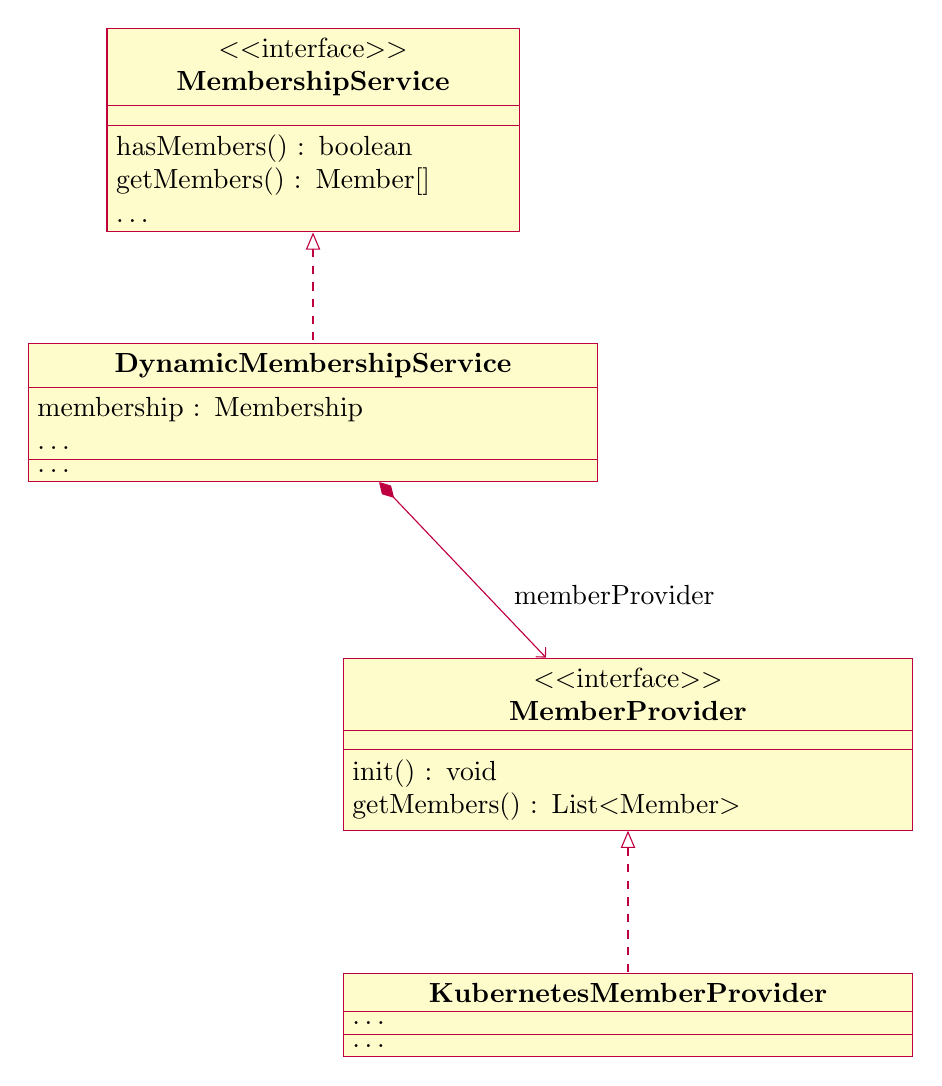
\begin{tikzpicture}
    \begin{interface}{MembershipService}{0,0}
      \operation{hasMembers() : boolean}
      \operation{getMembers() : Member[]}
      \operation{$\ldots$}
    \end{interface}

    \begin{class}[text width=7cm]{DynamicMembershipService}{0,-4}
      \implement{MembershipService}
      \attribute{membership : Membership}
      \operation{$\ldots$}
      \attribute{$\ldots$}
    \end{class}

    \begin{interface}[text width=7cm]{MemberProvider}{4,-8}
      \operation{init() : void}
      \operation{getMembers() : List\textless{}Member\textgreater{}}
    \end{interface}

    \begin{class}[text width=7cm]{KubernetesMemberProvider}{4,-12}
      \implement{MemberProvider}
      \operation{$\ldots$}
      \attribute{$\ldots$}
    \end{class}

    \composition{DynamicMembershipService}{memberProvider}{}{MemberProvider}
  \end{tikzpicture}

  \caption{Principal classes and interfaces in our implementation.}\label{fig:classes}
\end{figure}


\begin{figure}
  \centering

  \begin{sequencediagram}
    \newthread{rt}{RT}
    \newthread{dms}{DMS}
    \newinst[1]{mp}{MP}
    \newinst{m}{M}
    \newinst{ml}{ML}

    \begin{call}{dms}{init()}{mp}{}
    \end{call}

    \begin{call}{dms}{start()}{rt}{}
    \end{call}

    \begin{sdblock}{Main loop}{}
      \begin{call}{rt}{fetchMembers()}{dms}{}
        \begin{call}{dms}{getMembers()}{mp}{members}
        \end{call}

        \begin{sdblock}{loop}{[for each member]}
          \begin{call}{dms}{memberAlive(member)}{m}{isMemberAlive}
          \end{call}

          \begin{sdblock}{if}{[isMemberAlive]}
            \begin{call}{dms}{memberAdded(member)}{ml}{}
            \end{call}
          \end{sdblock}
        \end{sdblock}

      \begin{call}{dms}{expire()}{m}{expiredMembers}
      \end{call}

      \begin{sdblock}{loop}{[for each expiredMember]}
        \begin{call}{dms}{memberDisappeared(expiredMember)}{ml}{}
        \end{call}
      \end{sdblock}
    \end{call}
    \end{sdblock}
  \end{sequencediagram}

  \caption{Sequence diagram for \texttt{DynamicMembershipService} (DMS). The other actors are \texttt{RefreshThread} (RT), \texttt{MembershipProvider} (MP), \texttt{Membership} (M) and \texttt{MembershipListener} (ML)}\label{fig:seq}
\end{figure}


% ================================ %

\section{Testing}

During development, we needed a way to verify if session replication was working correctly. For this, we implemented a very simple test application that responds to HTTP requests with a JSON object containing following information:

\begin{itemize}
    \item A counter that is stored in a session and is upgraded at each request
    \item The current session ID
    \item A boolean, set to \texttt{true} if the session is freshly created
    \item The IP address and host name of the Tomcat instance that served the request
\end{itemize}

An example output is given in Listing~\ref{lst:example-output}

\begin{lstlisting}[caption=Example output,label=lst:example-output]
{
    "counter": 4,
    "id": "305F63E07385E9B2E434941DF607B60E",
    "new": false,
    "server": "172.17.0.2",
    "hostname": "tomcat-in-the-cloud-1-5xbwm"
}
\end{lstlisting}

By making multiple requests and checking if the counter is incremented, we can verify if sessions are correctly replicated regardless of the Tomcat instance that replied. In between requests, we scaled the number of instances up and down by running

\texttt{oc scale dc tomcat-in-the-cloud --replicas=\$N}

Where \texttt{\$N} is the desired number of instances. This allowed to verify that our solution was robust to churn (members joining and leaving the cluster).

The solution was tested successfully in two different OpenShift deployments:
\begin{itemize}
    \item On a 1-node OpenShift cluster, deployed by running \texttt{oc cluster up}
    \item On MiniShift\autocite{minishift}, an all-in-one solution for deploying a local OpenShift instance for testing purposes.
\end{itemize}

Unfortunately, we didn't have time to test our solution on a multi-node cluster, but we are confident that it would work just as well.

% ================================ %

\section{Issues and future improvements}

Although the solution is working as expected, some minor issues still exist.

\begin{itemize}
\item Error handling is at a bare minimum and should be improved.

\item The class \texttt{CertificateStreamProvider}\footnote{\url{https://github.com/jgroups-extras/jgroups-kubernetes/blob/master/src/main/java/org/jgroups/protocols/kubernetes/stream/CertificateStreamProvider.java}} isn't currently provided, as it wasn't needed in our test deployments and we wanted to avoid the additional \texttt{net.oauth} dependency.

\item Although the class is named \texttt{KubernetesMemberProvider}, it might not work in non-OpenShift Kubernetes installations, since the environment variables used to set up API calls might be different. Testing in such environments is required.

\item Multiple applications deployed to the same namespace/project will form a single cluster and share session data together, which adds some overhead (due to more data being shared) and can pose security risks. A solution to this could be possible with labels: \texttt{KubernetesMemberProvider} already filters pods by label if the environment variable \texttt{OPENSHIFT\_KUBE\_PING\_LABELS} is set (can be set in the file \emph{pom.xml}, similarly to \texttt{OPENSHIFT\_KUBE\_PING\_LABELS}), and labels can be added the application by fabric8\footnote{\url{https://maven.fabric8.io/\#resource-labels-annotations}}

\item Our testing method consisted of manually making requests and verifying that the counter was correctly incremented and that all the nodes were hit at least once. Instead, a script could be written to perform this task automatically. This script could even be extended to automatically scale the number of pods. Such a setup would help iterating faster.

\end{itemize}

% ================================ %

\clearpage
\appendix
\section{Usage instruction}\label{sec:usage}

Create a new OpenShift project or switch to an existing one: \\
\begin{lstlisting}
oc project tomcat-in-the-cloud
\end{lstlisting}

Authorize pods to see their peers: \\
\begin{lstlisting}
oc policy add-role-to-user view \
    system:serviceaccount:$(oc project -q):default \
    -n $(oc project -q)
\end{lstlisting}

Deploy your application: \\
\begin{lstlisting}
mvn fabric8:deploy
\end{lstlisting}

\subsection*{Customization}

\subsubsection*{Project name}

By default, the application is deployed to the project \emph{tomcat-in-the-cloud}. To change this, modify the value of \texttt{fabric8.namespace} in \emph{pom.xml}.

\subsubsection*{Server port}

Tomcat is set to listen to port 8080, and fabric8 must expose this port in the resulting containers. This value is specified in two places: in the application itself (see \emph{Main.java}), and in fabric8's configuration (variable \texttt{port} in \emph{pom.xml})

\subsubsection*{Number of replicas}

Upon deployment, the application is automatically scaled to 2 pods. This value can be changed in \emph{src/main/fabric8/deployment.yml}. When the default behavior (1 pod) is desired, this file can safely be deleted.

\subsubsection*{Sticky sessions}

To make testing easier, sticky sessions have been disabled in \emph{src/main/fabric8/route.yml}. To re-enable them, change \texttt{haproxy.router.openshift.io/disable\_cookies} to \texttt{true} or simply delete the file.

When making changes to the route configuration, run mvn fabric8:undeploy before deploying again to make sure that all changes are taken into account.

\clearpage
\printbibliography[heading=bibintoc]{}


\end{document}
